% ----------------------------------------------------------------------------
\chapter{Chat Protocol Definition}
    4. Protocol definition paper (containing chat features,
            data types, transport methods, security measures)
% ----------------------------------------------------------------------------
\section{Features}
This section describes which features are supported by the chat protocol.
Figure \ref{features-technologies} gives a quick overview of how the
features relate to the used technologies.
\begin{figure}
    \centering
    \caption{Features and Technologies}
    \label{features-technologies}
    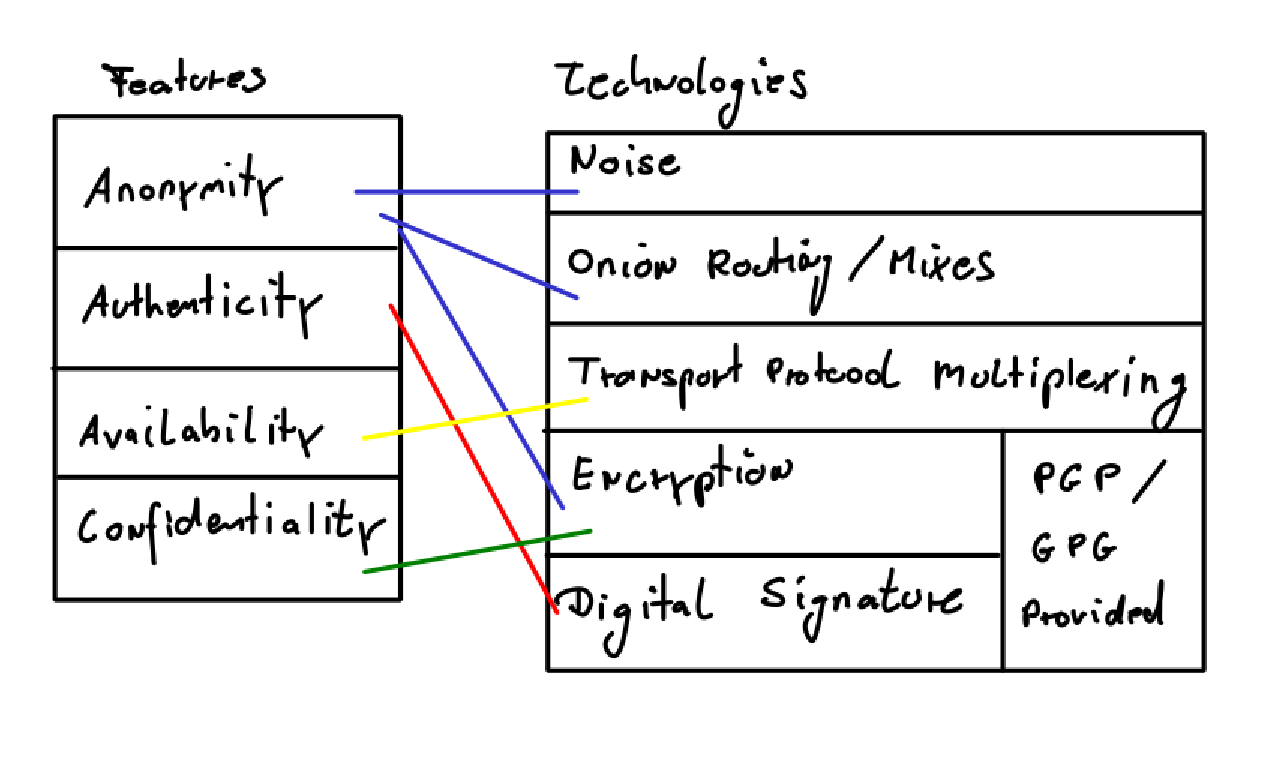
\includegraphics[scale=0.8]{features-technologies.eps}
\end{figure}
% ----------------------------------------------------------------------------
\subsection{Anonymity}
One of the main objectives of this thesis is to provide a chat system that
hides who is talking to whom (\textit{Sender-Receiver Anonymity}). 
In practise there are limits on the degree of anonymity that can be reached.


If an attacker controls all hosts that are 
part of the chat network, it is impossible to guarantee anonymity.

Thus the implementation should support be resistent against a high percentage
of attacker nodes in the network.

Level of anonymity in theory - nodes

Winning chances in Lotto are expressed like this:
$$P_r = \frac{{\binom{6}{r}}{\binom{N-6}{6-r}}}{{\binom{N}{6}}}, r \in \{0, \ldots, 6\}$$

To remove anonymity, all peers in a route, which are not the 
sender and the receiver have to be compromised.
Depending on the number of hosts in a network (number of possible
numbers in lotto) and on the number of hosts in a specific route
(number of correct numbers in lotto), the de-anonymisation
probalities (lotto: winning probabilities) are shown in table
\ref{deanontable}

%\begin{longtable}{|c|c|c|c|c|c|c|c|c|}
\begin{longtable}{|c|c|c|c|c|c|}
\caption{De-Anonymisation Probablities (for one packet)}
\label{deanontable}\\
\hline
\textbf{Peers in network /} & \textbf{$10$} & \textbf{$10^2$} & \textbf{$10^3$} & \textbf{$10^4$} & \textbf{$10^5$} \\
\textbf{Proxy peers} & & & & & \\
\hline
\textbf{1} & 1:10 & 1:100 & 1:1000 & 1:10000 & 1:100000\\
\hline
\textbf{2} & 1:45 & 1:4950 & 1:499500 & 1:4.9995e+07 & 1:4.99995e+09\\
\hline
\textbf{3} & 1:120 & 1:161700 & 1:1.66167e+08 & 1:1.66617e+11 & 1:1.66662e+14\\
\hline
\textbf{4} & 1:210 & 1:3.92122e+06 & 1:4.14171e+10 & 1:4.16417e+14 & 1:4.16642e+18\\
\hline
\textbf{5} & 1:252 & 1:7.52875e+07 & 1:8.25029e+12 & 1:8.325e+17 & 1:8.3325e+22\\
\hline
\textbf{6} & 1:210 & 1:1.19205e+09 & 1:1.36817e+15 & 1:1.38681e+21 & 1:1.38868e+27\\
\hline
\textbf{7} & 1:120 & 1:1.60076e+10 & 1:1.94281e+17 & 1:1.97996e+24 & 1:1.98371e+31\\
\hline
\textbf{8} & 1:45 & 1:1.86088e+11 & 1:2.41151e+19 & 1:2.47322e+27 & 1:2.47946e+35\\
\hline
\textbf{9} & 1:10 & 1:1.90223e+12 & 1:2.65802e+21 & 1:2.74583e+30 & 1:2.75474e+39\\
\hline
\textbf{10} & 1:1 & 1:1.73103e+13 & 1:2.6341e+23 & 1:2.74336e+33 & 1:2.75449e+43\\
\hline
\end{longtable}

% ----------------------------------------------------------------------------
\subsection{Authenticity}
Digital signatures provide methods to ensure that a given message
was composed by a given public key and that the content has not been
modified.
% ----------------------------------------------------------------------------
\subsection{Confidentiality}
The process of encryption protects data and thus ensures the
confidentiality of a message.
% ----------------------------------------------------------------------------
\subsection{Availability}
% ----------------------------------------------------------------------------
\subsection{Non security related features}
This chat protocol version supports only direct chat as opposed to
multi user / group chat.
% ----------------------------------------------------------------------------
\section{Encryption and Digital Signature}
Message encryption and digital signatures are
used as defined in the OpenPGP RFC.\cite{rfc2440}


% ----------------------------------------------------------------------------
\section{Onion Routing}

% ----------------------------------------------------------------------------
\section{Transport protocols}
 /  Inter Machine Protocol

On the "`wire"'. Different transports. Constant transport.
Define name (postcard?!) here. Includes transport specific
header / meta information.

% ----------------------------------------------------------------------------
\subsection{Tunneling}
aginst firewall rules / blocking of traffic
through http
steganographic

% ----------------------------------------------------------------------------
\subsection{Multiplexing}
\subsubsection{Variable Transports}
Different transports for one peer.
% ----------------------------------------------------------------------------
\subsection{List of Supported Transports}
To ensure interoperability, clients which support a specific
protocol version must support all listed transport protocols.
\begin{longtable}{|c|c|c|}
\caption{Transport protocols}\\
\hline
\textbf{Protocol} & \textbf{Description} & \textbf{Supported versions}\\
\hline
tcp & Transmission Control Protocol & 0.1 - 0.1\\
\hline
\end{longtable}

\subsubsection{Variable Peers}
Different routes for every packet
\subsubsection{Constant sending}

\subsubsection{Source based routing}
Either here or in Intra Machine Intra Client
\subsubsection{Peer selection}
Which peers, how many. Constant? May give upper bounds of latency.

8 * 0.5seconds = 4 seconds delay.

% ----------------------------------------------------------------------------
\section{Noise}
% ----------------------------------------------------------------------------
\subsection{Noise}

The average latency for a peer is calculated as follows:
$$\frac{\sum\limits_{i=0}^{(Proxy peers +1)}}{Proxy peers + 1}$$
Depending on how long the waiting delay in seconds is, this results
in different average waiting times for message to arrive, as expressed in
the following formula:
$$Delaytime * \frac{\sum\limits_{i=0}^{(Proxy peers +1)}}{Proxy peers + 1}$$

\begin{longtable}{|c|c|c|c|c|c|c|}
\caption{Average latency based on number of proxy peers}
\label{avglatencypeers}\\
\hline
\multirow{2}{*}{\textbf{Proxy peers}} & \multicolumn{6}{|l|}{\textbf{Average latency (multiplied by delay times)}} \\
& \textbf{(\# timeslots)} & \textbf{0.125s} & \textbf{0.25s} & \textbf{0.5s} & \textbf{1s} & \textbf{2s}\\
\hline
\textbf{1} & 0.5 & 0.0625s & 0.125s & 0.25s & 0.5s & 1s\\
\hline
\textbf{2} & 1 & 0.125s & 0.25s & 0.5s & 1s & 2s\\
\hline
\textbf{3} & 1.5 & 0.1875s & 0.375s & 0.75s & 1.5s & 3s\\
\hline
\textbf{4} & 2 & 0.25s & 0.5s & 1s & 2s & 4s\\
\hline
\textbf{5} & 2.5 & 0.3125s & 0.625s & 1.25s & 2.5s & 5s\\
\hline
\textbf{6} & 3 & 0.375s & 0.75s & 1.5s & 3s & 6s\\
\hline
\textbf{7} & 3.5 & 0.4375s & 0.875s & 1.75s & 3.5s & 7s\\
\hline
\textbf{8} & 4 & 0.5s & 1s & 2s & 4s & 8s\\
\hline
\textbf{9} & 4.5 & 0.5625s & 1.125s & 2.25s & 4.5s & 9s\\
\hline
\textbf{10} & 5 & 0.625s & 1.25s & 2.5s & 5s & 10s\\
\hline
\end{longtable}
A study about 
\textit{System Response Time and User Satisfaction}\cite{responsetime}
indicates that response times up to 6 seconds are tolerable, these numbers
cannot be related directly to the tolerated delay, because the receiving
peer does not know when the sending peer sent a message.

\begin{longtable}{|c|c|c|c|c|c|c|}
\caption{Maximum latency based on number of proxy peers}
\label{maxlatencypeers}\\
\hline
\multirow{2}{*}{\textbf{Proxy peers}} & \multicolumn{6}{|l|}{\textbf{Maximum latency (multiplied by delay times)}} \\
& \textbf{(\# timeslots)} & \textbf{0.125s} & \textbf{0.25s} & \textbf{0.5s} & \textbf{1s} & \textbf{2s}\\
\hline
\textbf{1} & 1 & 0.125s & 0.25s & 0.5s & 1s & 2s\\
\hline
\textbf{2} & 2 & 0.25s & 0.5s & 1s & 2s & 4s\\
\hline
\textbf{3} & 3 & 0.375s & 0.75s & 1.5s & 3s & 6s\\
\hline
\textbf{4} & 4 & 0.5s & 1s & 2s & 4s & 8s\\
\hline
\textbf{5} & 5 & 0.625s & 1.25s & 2.5s & 5s & 10s\\
\hline
\textbf{6} & 6 & 0.75s & 1.5s & 3s & 6s & 12s\\
\hline
\textbf{7} & 7 & 0.875s & 1.75s & 3.5s & 7s & 14s\\
\hline
\textbf{8} & 8 & 1s & 2s & 4s & 8s & 16s\\
\hline
\textbf{9} & 9 & 1.125s & 2.25s & 4.5s & 9s & 18s\\
\hline
\textbf{10} & 10 & 1.25s & 2.5s & 5s & 10s & 20s\\
\hline
\end{longtable}


% ----------------------------------------------------------------------------
\subsection{Bandwidth usage}
\begin{verbatim}
>>> messages_size=4*1024
>>> messages_per_second=4
>>> bytes_per_second=messages_per_second*messages_size
>>> print(bytes_per_second)
16384
>>> bytes_per_day=86400*bytes_per_second
>>> print(bytes_per_day)
1415577600
>>> print(bytes_per_day/1024**2)
1350.0
>>> bytes_per_month=month_length*bytes_per_day
>>> print(bytes_per_month/1024**2)
41062.5
>>> print(bytes_per_month/1024**3)
40.10009765625
\end{verbatim}
16 KiB/s or 128 KBit/s, 2 ISDN lines. Around 1.4 GiB per day or
circa 40 GiB per month.

% ----------------------------------------------------------------------------
\subsection{Inter Machine Inter Program Protocol}
After decoding the received packet. Forward, etc.
Based on part os EOF simple data types.
\subsubsection{Message types}
List of messages here
\subsubsection{Message 1}
description here

% ----------------------------------------------------------------------------
\subsection{Version}
As soon as this standard is usable and the first version of \emph{rEOFi}
is released, it will version number \textbf{01} of the standard.
Further changes will be documented in this section. All version numbers
are two ASCII digits (see below).
% Nico: FIXME for 1.0

% Nico: 1.0
% #############################################################################
